\section{Imputering og ekstrapolering}

% \begin{frame}{Imputering og ekstrapolering}
%     \textbf{Manglende observationer i paneldatasættene:}
%     \begin{itemize}
%       \item Alle år mangler observationer for et flertal af vandområder.
%       \item Overvågningen er ikke sket mhp. repræsentativitet.
%       \item Der er overrepræsentation af større vandområder samt vandområder med særlig grund til bekymring.
%     \end{itemize}
%     \vfill
% \end{frame}
% \begin{frame}{Imputering og ekstrapolering}
%   \textbf{Manglende observationer i paneldatasættene:}
%   \begin{itemize}
%     \item Alle år mangler observationer for et flertal af vandområder.
%     \item Overvågningen er ikke sket mhp. repræsentativitet.
%     \item Der er overrepræsentation af større vandområder samt vandområder med særlig grund til bekymring.
%   \end{itemize}
%   \textbf{Imputering:}
%   \begin{itemize}
%     \item Manglende observationer estimeres vha. \textit{multivariate imputation by chained equations (MICE)}, hvor en \textit{fully conditional specification (FCS)} udgøres af en betinget densitet for hvert år.
%     \item Fysiske karakteristika inkluderes i \textit{Bayesian ridge regression} ved \textit{iteratively-reweighted regularized least-squares}.
%   \end{itemize}
%   \vfill
% \end{frame}
\begin{frame}{Imputering og ekstrapolering}
  \textbf{Manglende observationer i paneldatasættene:}
  \begin{itemize}
    \item Alle år mangler observationer for et flertal af vandområder.
    \item Overvågningen er ikke sket mhp. repræsentativitet.
    \item Der er overrepræsentation af større vandområder samt vandområder med særlig grund til bekymring.
  \end{itemize}
  \textbf{Imputering:}
  \begin{itemize}
    \item Manglende observationer estimeres vha. \textit{multivariate imputation by chained equations (MICE)}, hvor en \textit{fully conditional specification (FCS)} udgøres af en betinget densitet for hvert år.
    \item Fysiske karakteristika inkluderes i \textit{Bayesian ridge regression} ved \textit{iteratively-reweighted regularized least-squares}.
  \end{itemize}
  \textbf{Ekstrapolering af vandløbs tilstand til 1990 og 1991:}
  \begin{itemize}
    \item Estimeres ved at estimere en lineær trend og forlænge den.
  \end{itemize}
\end{frame}

% \begin{frame}{Vandløb: Sammensætning af smådyr (DVFI)}
%   \begin{itemize}
%     \item 17,933 km vandløb i VP2. 91\% er undersøgt mindst én gang.
%     \item Hvert år er 24\% undersøgt i gennemsnit (1992-2019).
%   \end{itemize}
%   \vfill
% \end{frame}
\begin{frame}{Vandløb: Sammensætning af smådyr (DVFI)}
  \begin{itemize}
    \item 17,933 km vandløb i VP2. 91\% er undersøgt mindst én gang.
    \item Hvert år er 24\% undersøgt i gennemsnit (1992-2019).
  \end{itemize}
  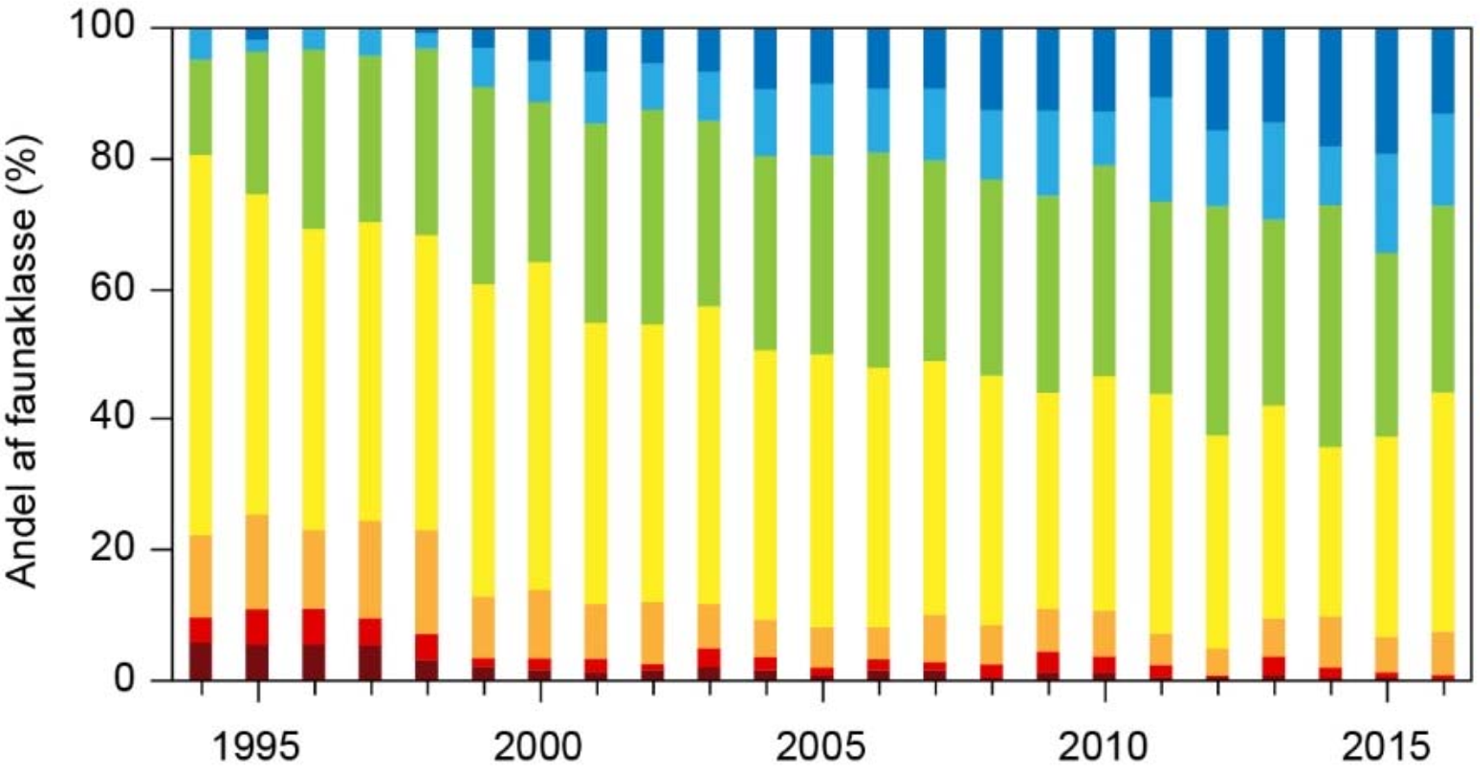
\includegraphics[width=\textwidth]{figures/DVFI}
\end{frame}

% \begin{frame}{Søer $>$ 5 ha: Klorofyl \textit{a}}
%   \begin{itemize}
%     \item 180 søer med faste kontroller.
%     \item 447 søer med enkelte operationelle overvågninger.
%   \end{itemize}
%   \vfill
% \end{frame}
\begin{frame}{Søer $>$ 5 ha: Klorofyl \textit{a}}
  \begin{itemize}
    \item 180 søer med faste kontroller.
    \item 447 søer med enkelte operationelle overvågninger.
  \end{itemize}
  Kerne af 29 søer med mange kontroller siden 1989:
  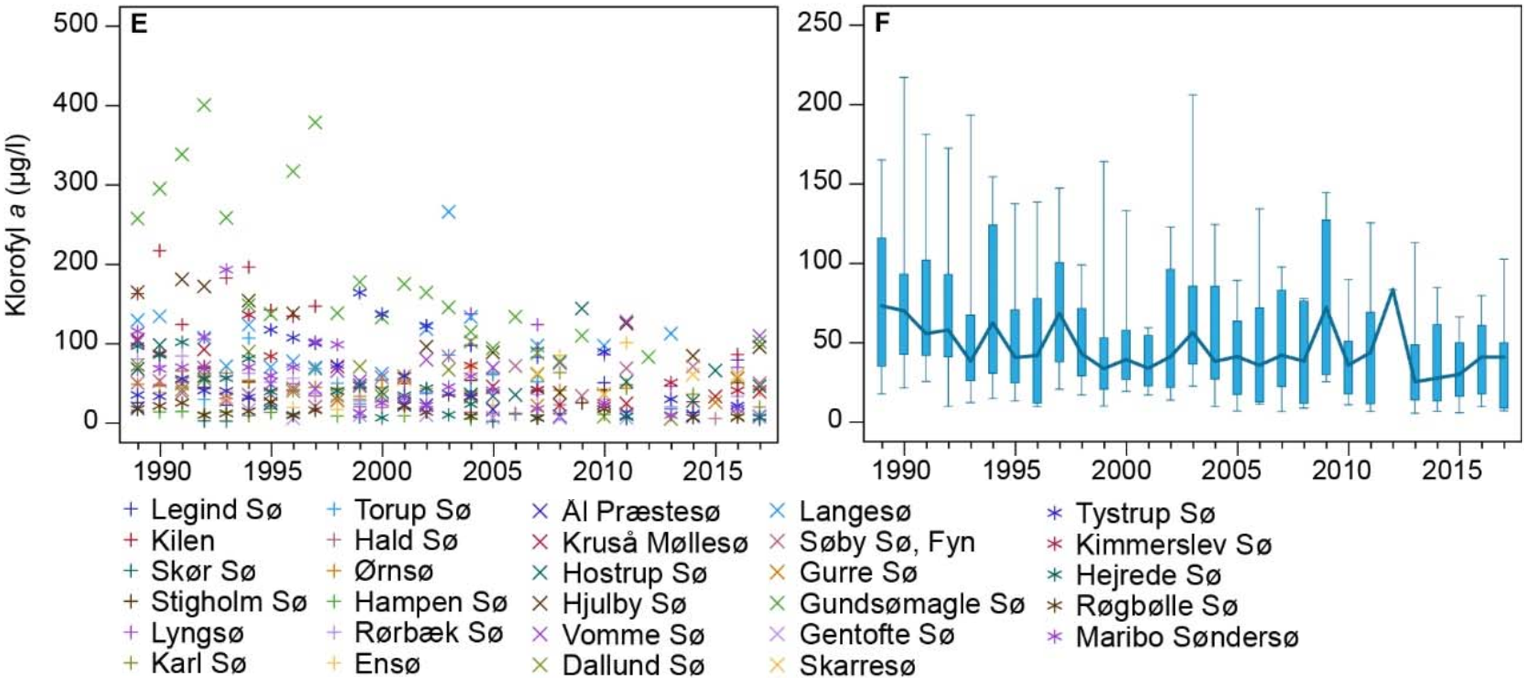
\includegraphics[width=\textwidth]{figures/chlorophyll_lakes}
\end{frame}

\begin{frame}{Fjorde og kystvande: Klorofyl \textit{a}}
  \begin{itemize}
    \item Klorofyl (planteplankton) er målt hvert sommer siden 1989.
  \end{itemize}
  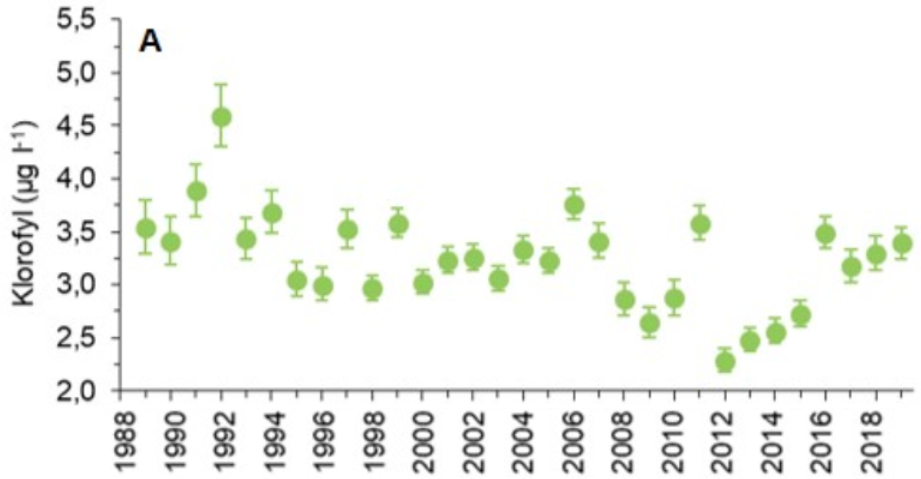
\includegraphics[width=\textwidth]{figures/chlorophyll_fjords_coastal}
\end{frame}

\begin{frame}{Fjorde og kystvande: Dybdegrænse for ålegræs}
  \begin{itemize}
    \item Dybdegrænsen for ålegræssets maksimale udbredelse måles minimum hvert 3. år.
  \end{itemize}
  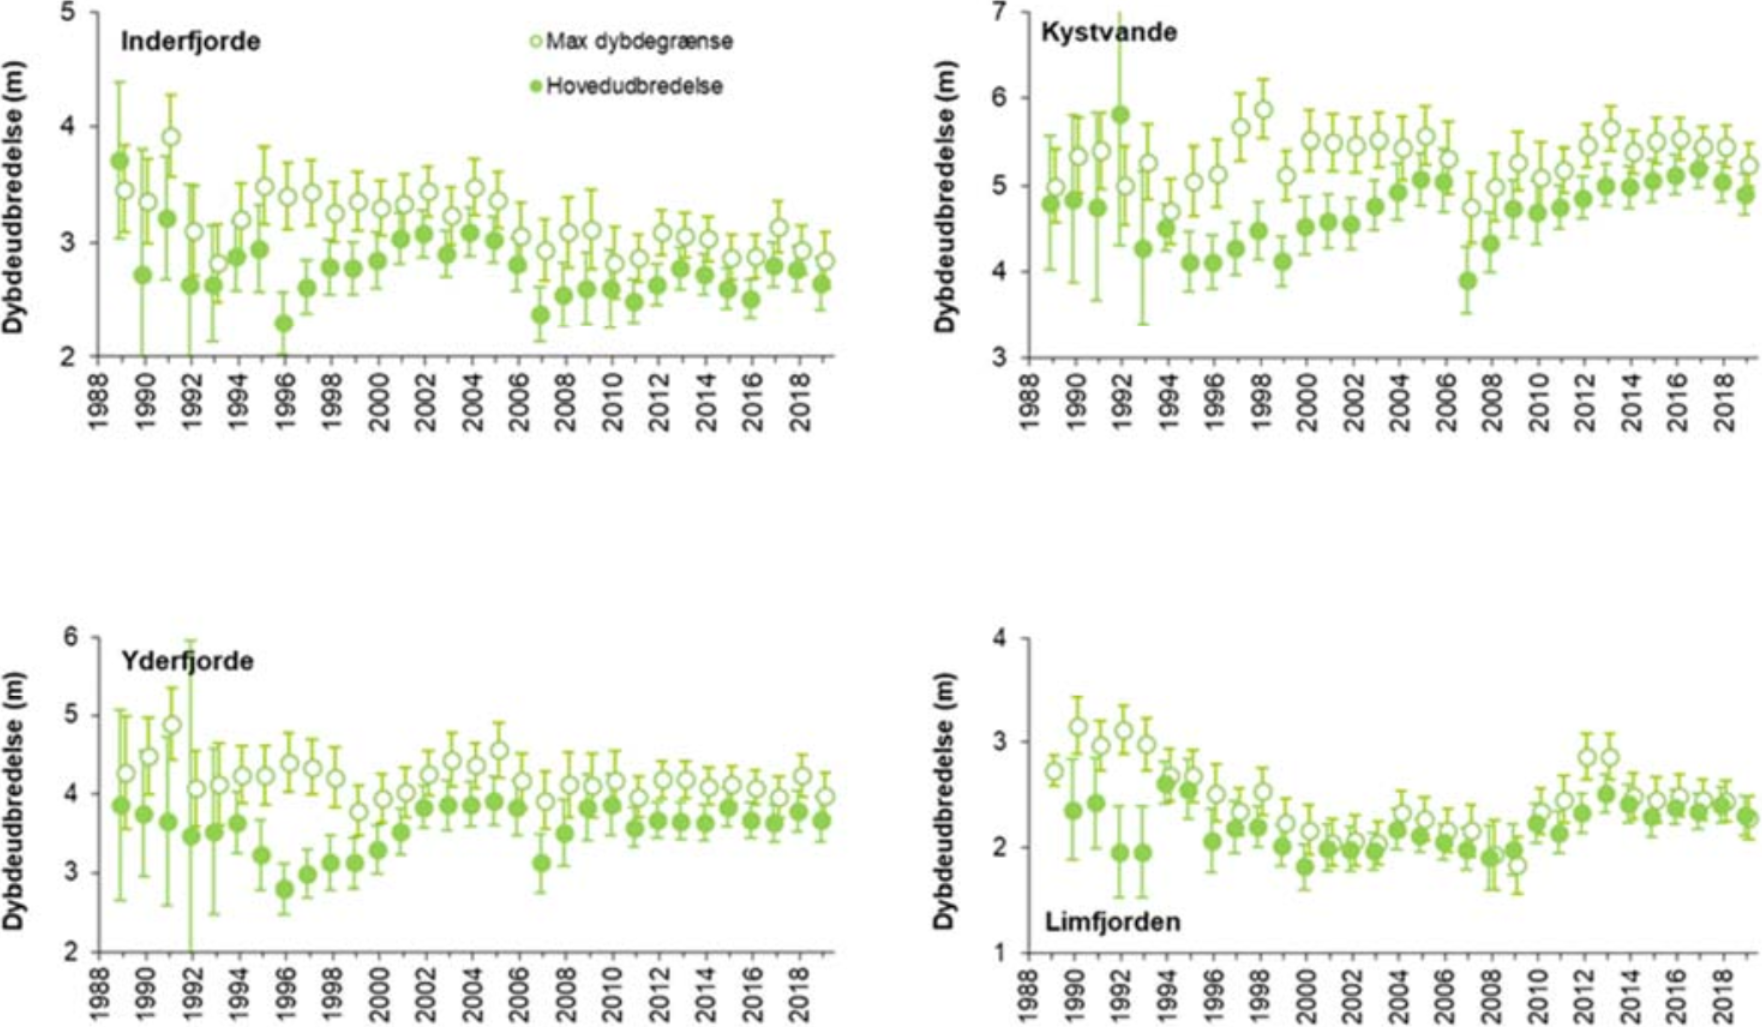
\includegraphics[width=\textwidth]{figures/eelgrass}
\end{frame}
